\documentclass[aspectratio=169]{beamer}
%\usetheme{CambridgeUS}
%\usecolortheme{beaver}

%\usefonttheme{serif}
%\usepackage{helvet}

\usefonttheme{serif}     % Font theme: serif
%\usepackage{ccfonts}     % Font family: Concrete Math
\usepackage[T1]{fontenc} % Font encoding: T1

\setbeamersize{text margin left=42pt,text margin right=42pt} 
\setbeamertemplate{navigation symbols}{}
\setbeamertemplate{itemize items}[default]

\beamertemplatenavigationsymbolsempty

\definecolor{fore}{RGB}{51,51,51}
\definecolor{back}{RGB}{255, 254, 250}
\definecolor{title}{RGB}{ 255, 15, 0}
\definecolor{links}{RGB}{18, 168, 255}

\setbeamercolor{titlelike}{fg=title}
\setbeamercolor{normal text}{fg=fore,bg=back}
\setbeamercolor{alerted text}{fg=title}
\setbeamercolor{itemize item}{fg=title}
\setbeamercolor{enumerate item}{fg=title}
\hypersetup{colorlinks,urlcolor=links}

% for code https://kbroman.org/blog/2013/10/07/better-looking-latexbeamer-slides/
\usepackage{listings}
\definecolor{keywords}{RGB}{255,0,90}
\definecolor{comments}{RGB}{60,179,113}
\lstset{language=Python,
keywordstyle=color{keywords},
commentstyle=color{comments}emph}

% fonts
\usepackage[sc]{mathpazo}


% title info
\title{\textbf{Cycling \& Walking:}}
\subtitle{\textbf{GGR424 - Transportation Geography \& Planning}}
\author{Jeff Allen}
\institute{University of Toronto}
\date{January 24, 2022}


\begin{document}
	
\begin{frame}
	\titlepage	
\end{frame}




\begin{frame}
	\begin{columns}
		\begin{column}{0.5\textwidth}
			
			\textbf{Today:}
			\begin{itemize}
				\item Benefits of active travel
				
				\item Safety issues and other concerns
				
				\item Designing safer infrastructure
				
				\item Designing "complete streets"
				
				\item Networks \& connectivity
			\end{itemize}
			
		\end{column}
		
		\begin{column}{0.5\textwidth}
			\begin{figure}
				\centering
				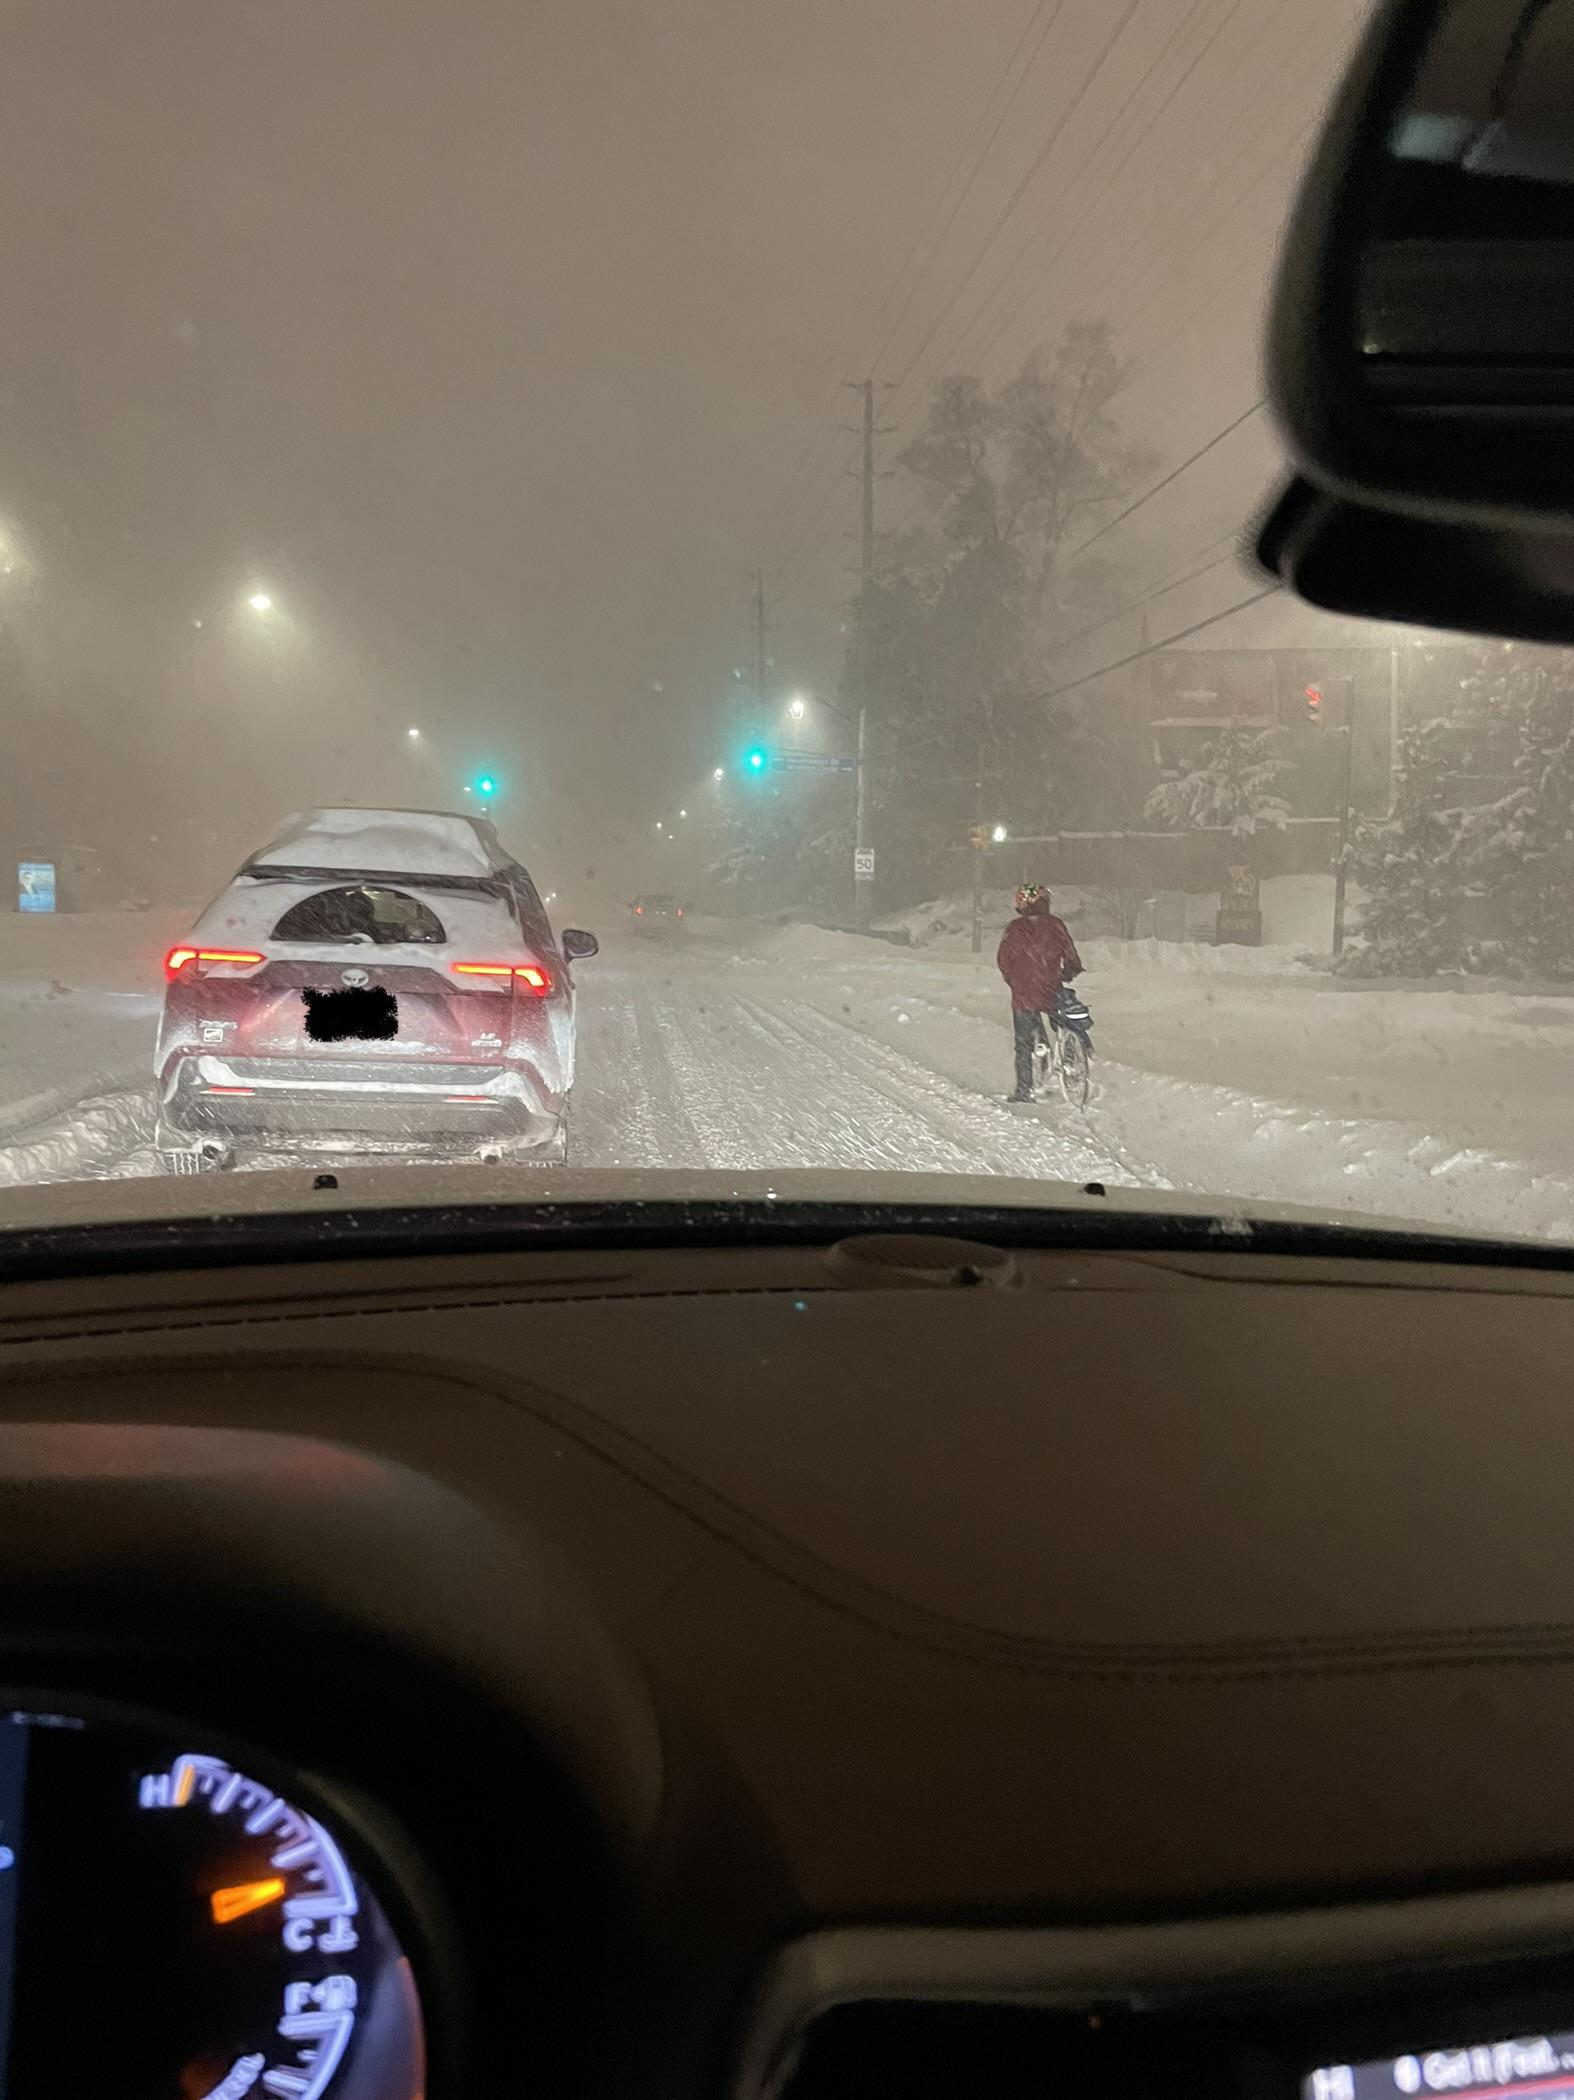
\includegraphics[width=0.8\linewidth]{images/bike_winter.jpg}
			\end{figure}
			
		\end{column}
		
		
		
	\end{columns}
\end{frame}




\begin{frame}
	
	\textbf{Active travel} - non-motorized mobility
	
	\vspace{2mm}
	
	e.g. walking and cycling, but also rollerblading, skateboarding, ice-skating, kick scooters, cross-country skiing, etc.
	
	\vspace{2mm}
	
	Can be for travelling to a specific location, or recreational travel not directed to a particular destination 

	\begin{figure}
		\centering
		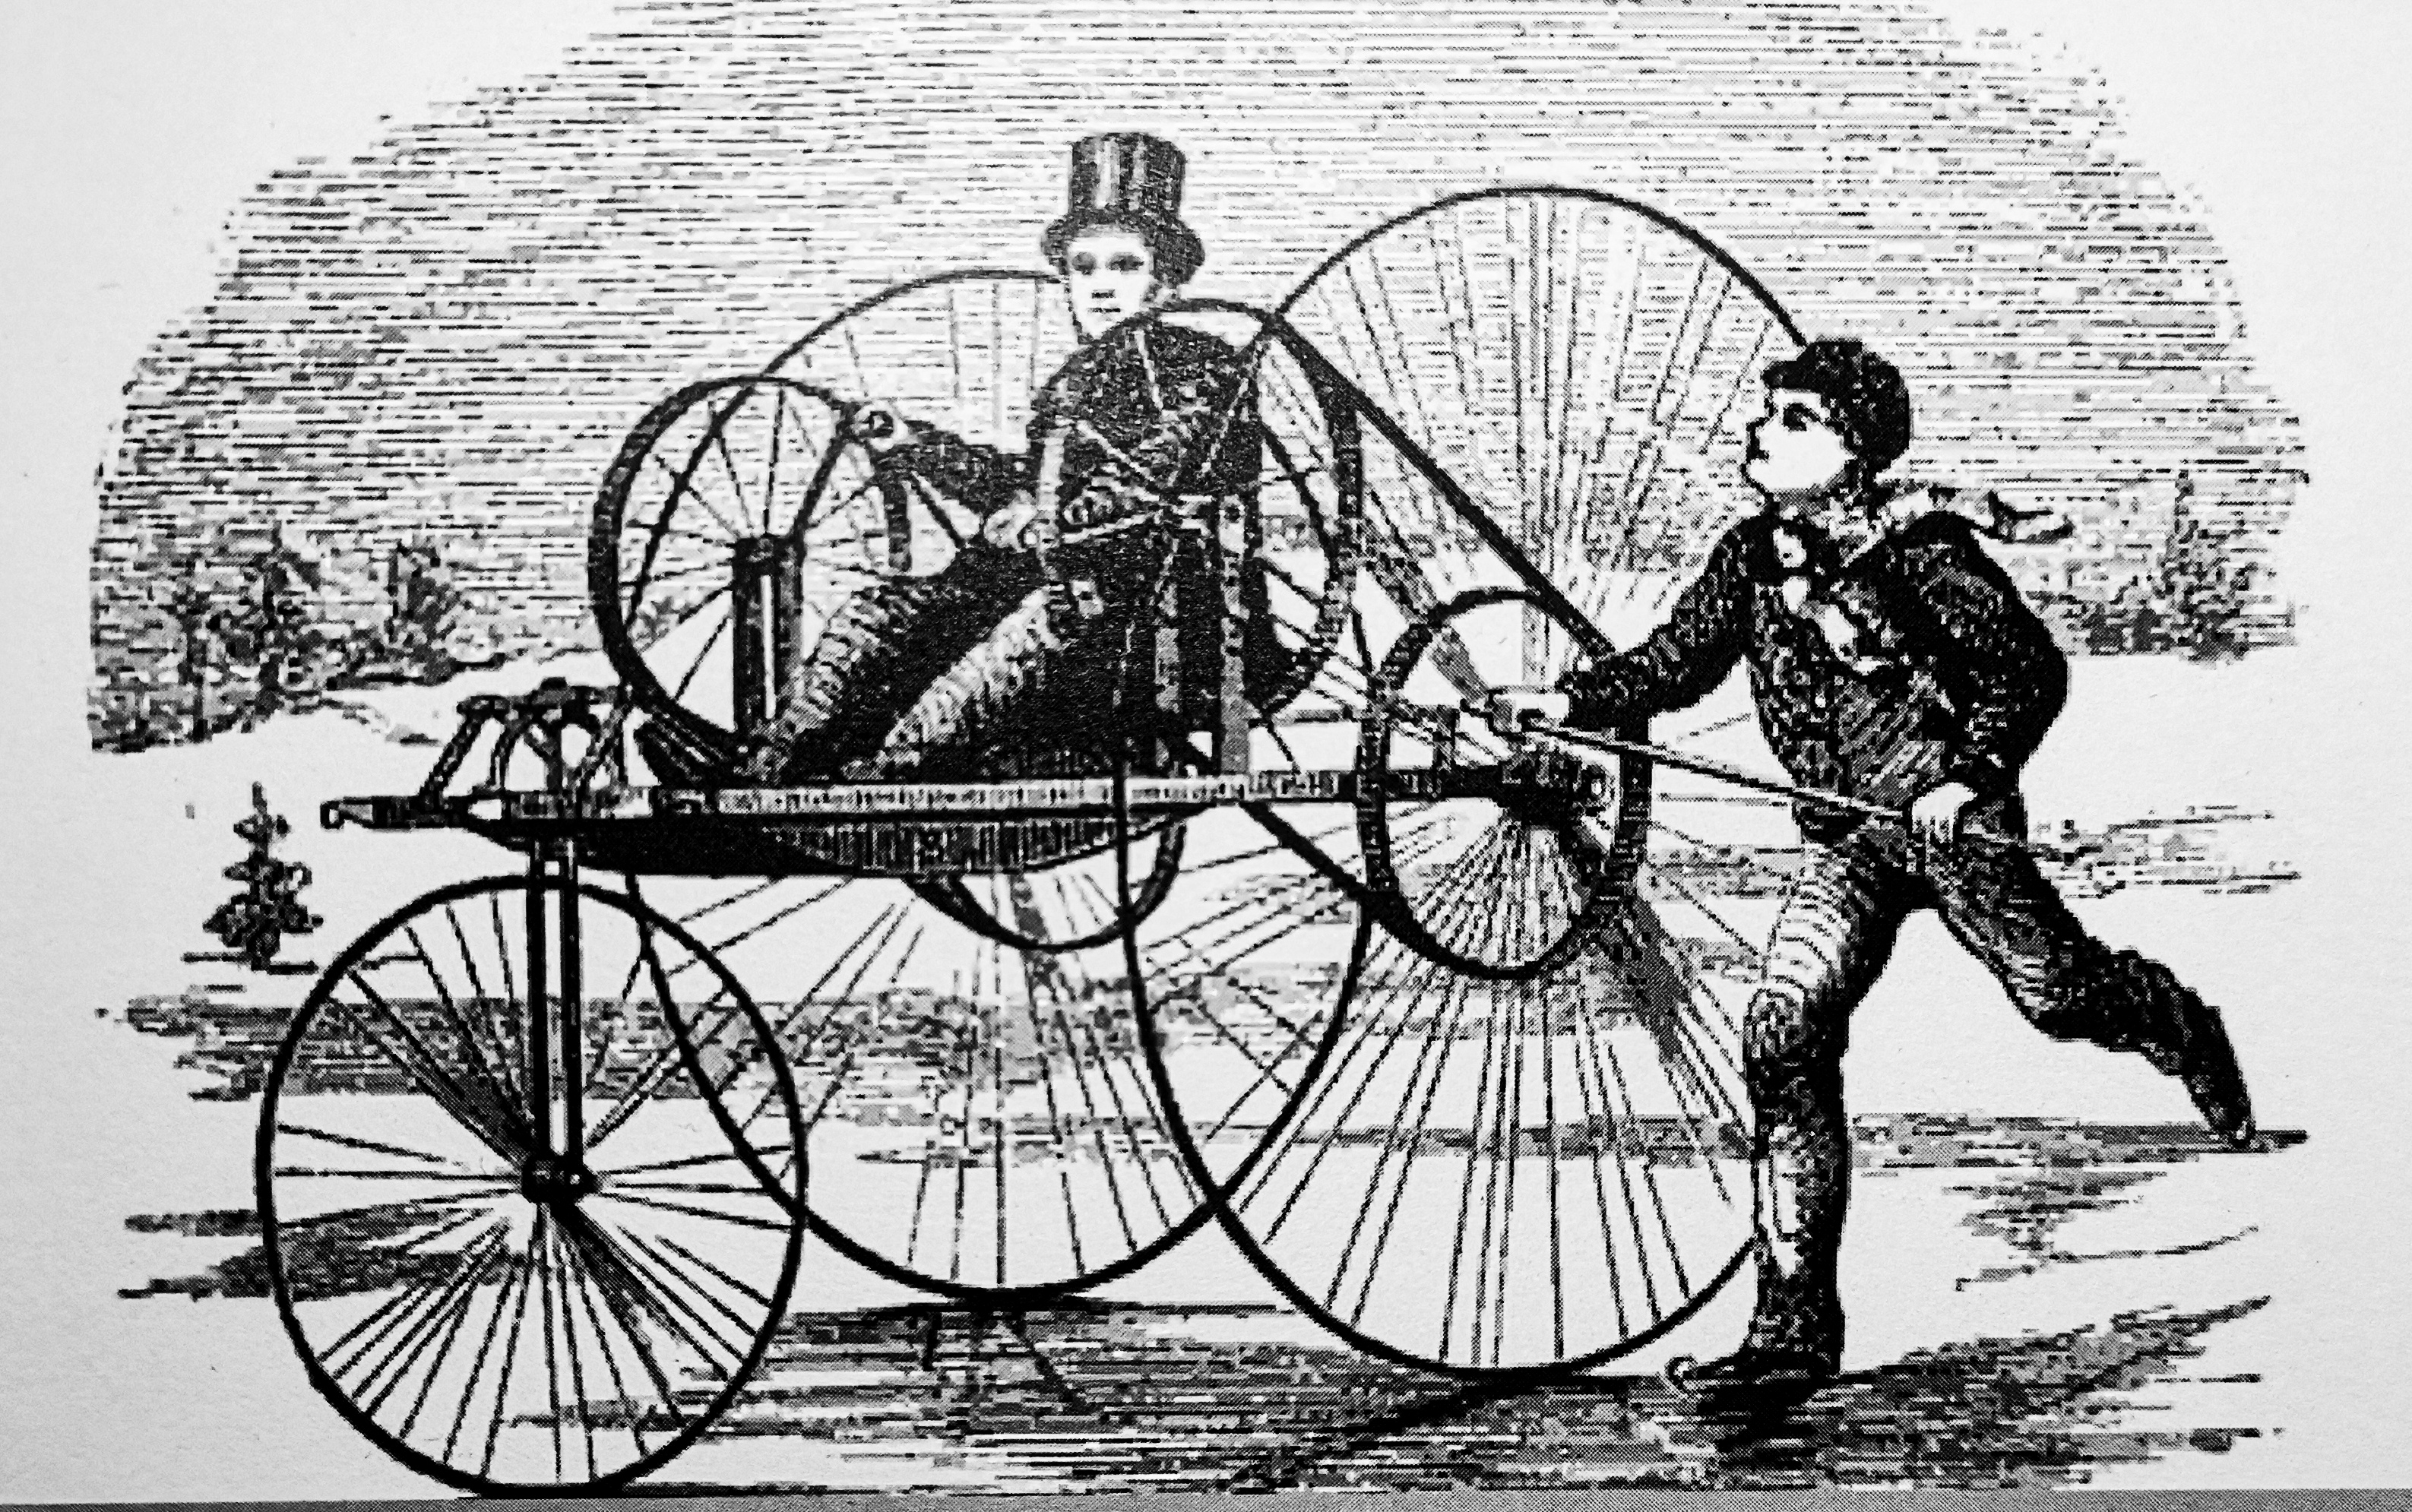
\includegraphics[width=0.55\linewidth]{images/velocipede.jpg}
	\end{figure}
		
\end{frame}




\begin{frame}
	
	\textbf{Benefits of Active Travel}
	
	\vspace{4mm}
	
	Can replace trips by other modes (driving, transit), meaning reduced congestion, pollution, GHG emissions, etc.
	
	\begin{figure}
		\centering
		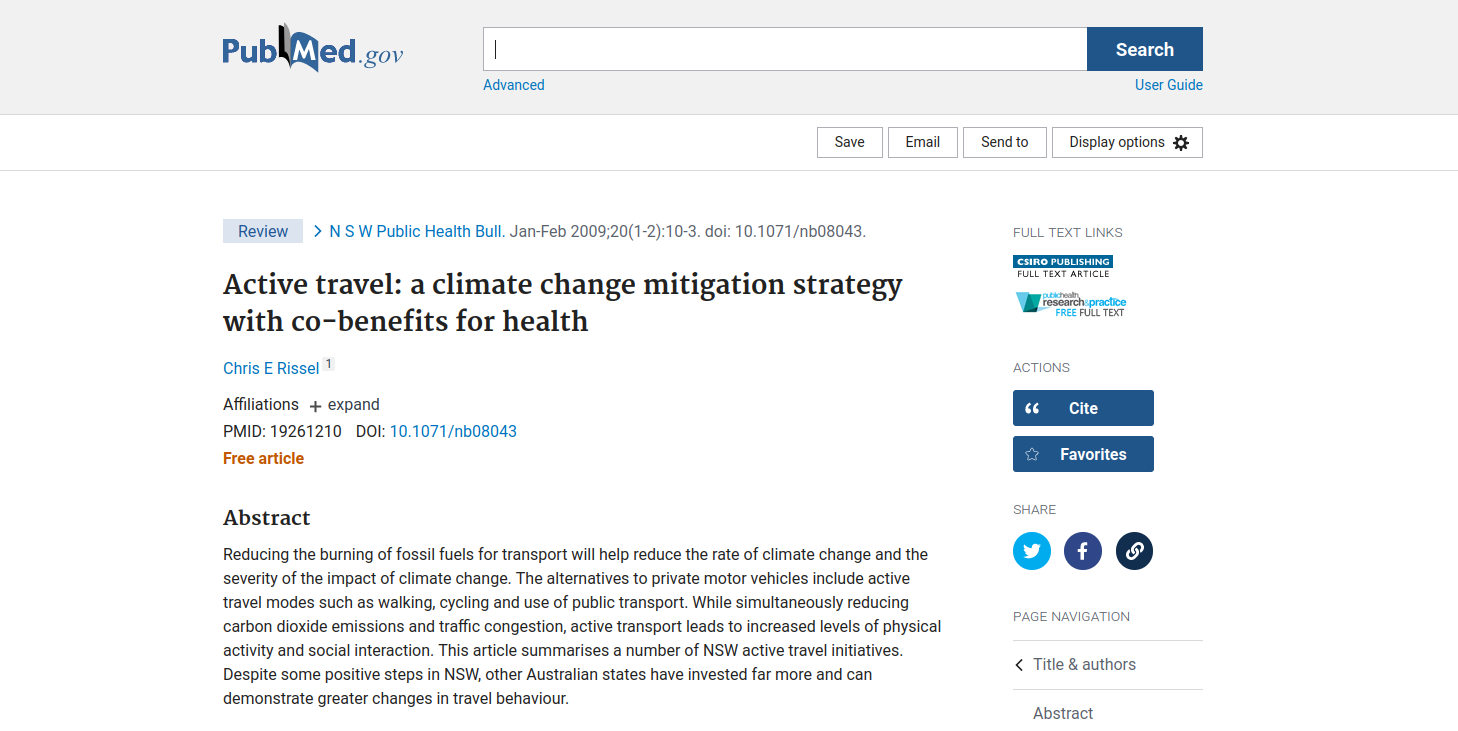
\includegraphics[width=0.7\linewidth]{images/active_travel_pollution.png}
	\end{figure}
	
	\tiny\url{https://pubmed.ncbi.nlm.nih.gov/19261210/}

\end{frame}



\begin{frame}
	
	\textbf{Benefits of Active Travel}
	
	\vspace{4mm}
	
	Plenty of research highlights health benefits of active travel, e.g. 
	
	\begin{figure}
		\centering
		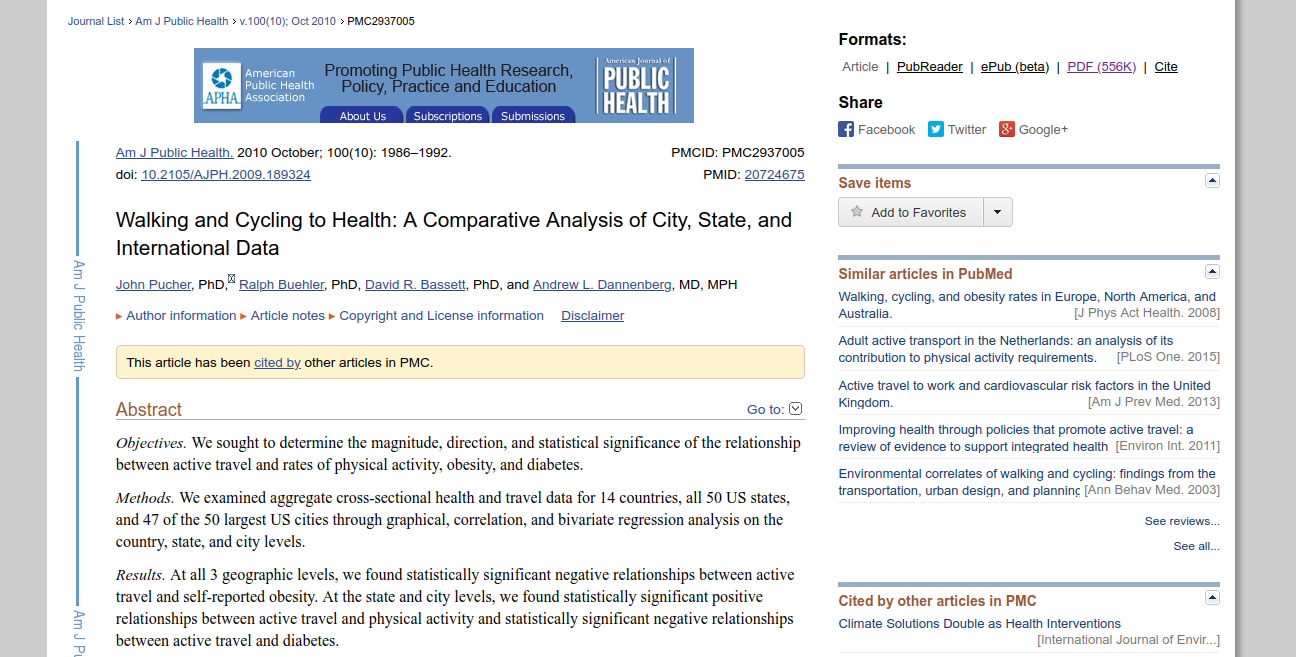
\includegraphics[width=1\linewidth]{images/health_ben_active_travel.png}
	\end{figure}
	
\end{frame}




\begin{frame}
	
	\textbf{Benefits of Active Travel}
	
	\vspace{4mm}
	
	Increased "enjoyment" or "satisfaction" of travel
	
	\begin{figure}
		\centering
		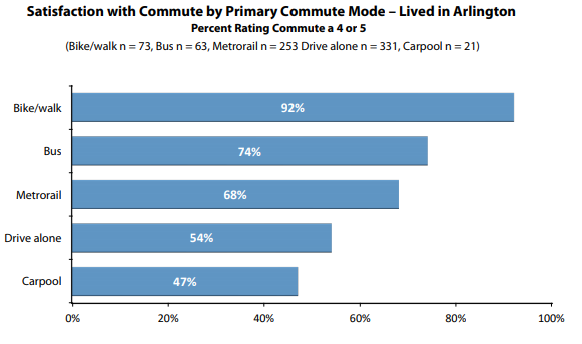
\includegraphics[width=0.7\linewidth]{images/mode_satisfaction.png}
	\end{figure}

	\tiny\url{https://mobilitylab.org/2020/09/29/the-pursuit-of-happiness-how-commute-mode-affects-commute-mood/}
	
\end{frame}



\begin{frame}
	
	\textbf{Benefits of Active Travel}
	
	\vspace{4mm}
	
	\small{"studies indicate that creating or improving active travel facilities generally has positive or non-significant economic impacts on retail"}
	
	\begin{figure}
		\centering
		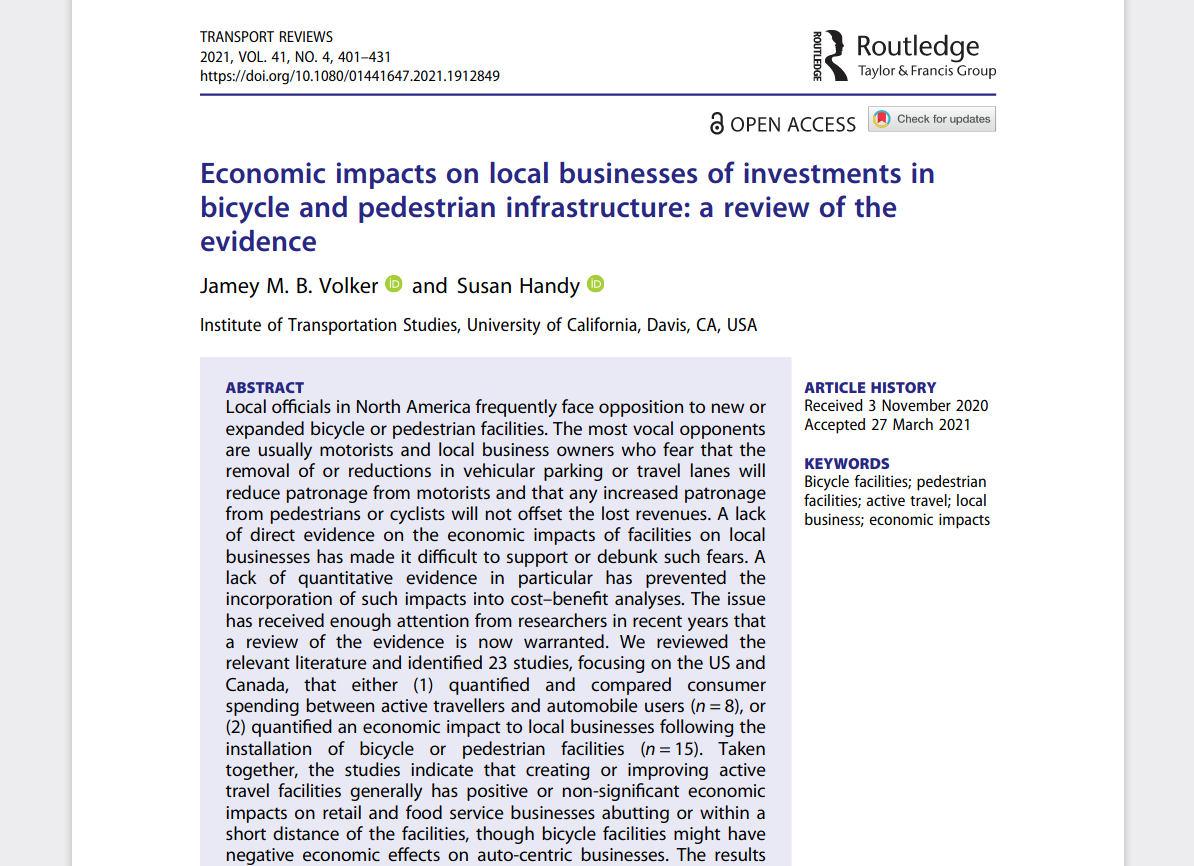
\includegraphics[width=0.6\linewidth]{images/economic_impacts_active_travel.png}
	\end{figure}
	
	\tiny\url{https://doi.org/10.1080/01441647.2021.1912849}
	
\end{frame}








\begin{frame}
	\begin{columns}
		\begin{column}{0.5\textwidth}
			
			\textbf{What deters active travel?}
			
			\vspace{8mm}
			
			\tiny{Image by Karl Jilg, commissioned by the Swedish Road Administration in 2014}
				
			\tiny\url{https://archive.attn.com/stories/17066/illustration-nails-pedestrian-problem-cities}
			
		\end{column}
		
		\begin{column}{0.5\textwidth}
			\begin{figure}
				\centering
				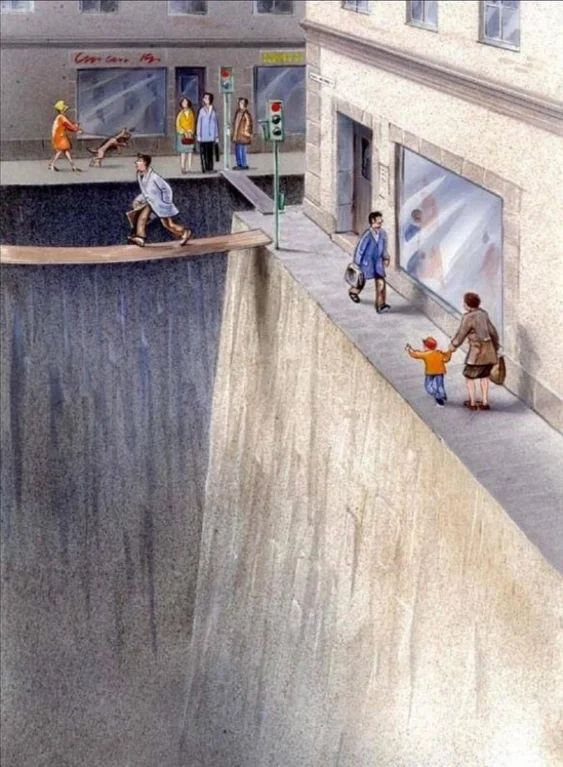
\includegraphics[width=0.9\linewidth]{images/deter_active_travel.jpg}
			\end{figure}
			
		\end{column}
		
		
		
	\end{columns}
\end{frame}




\begin{frame}
	
	\textbf{Induced demand, not just for cars!}
	
	\begin{figure}
		\centering
		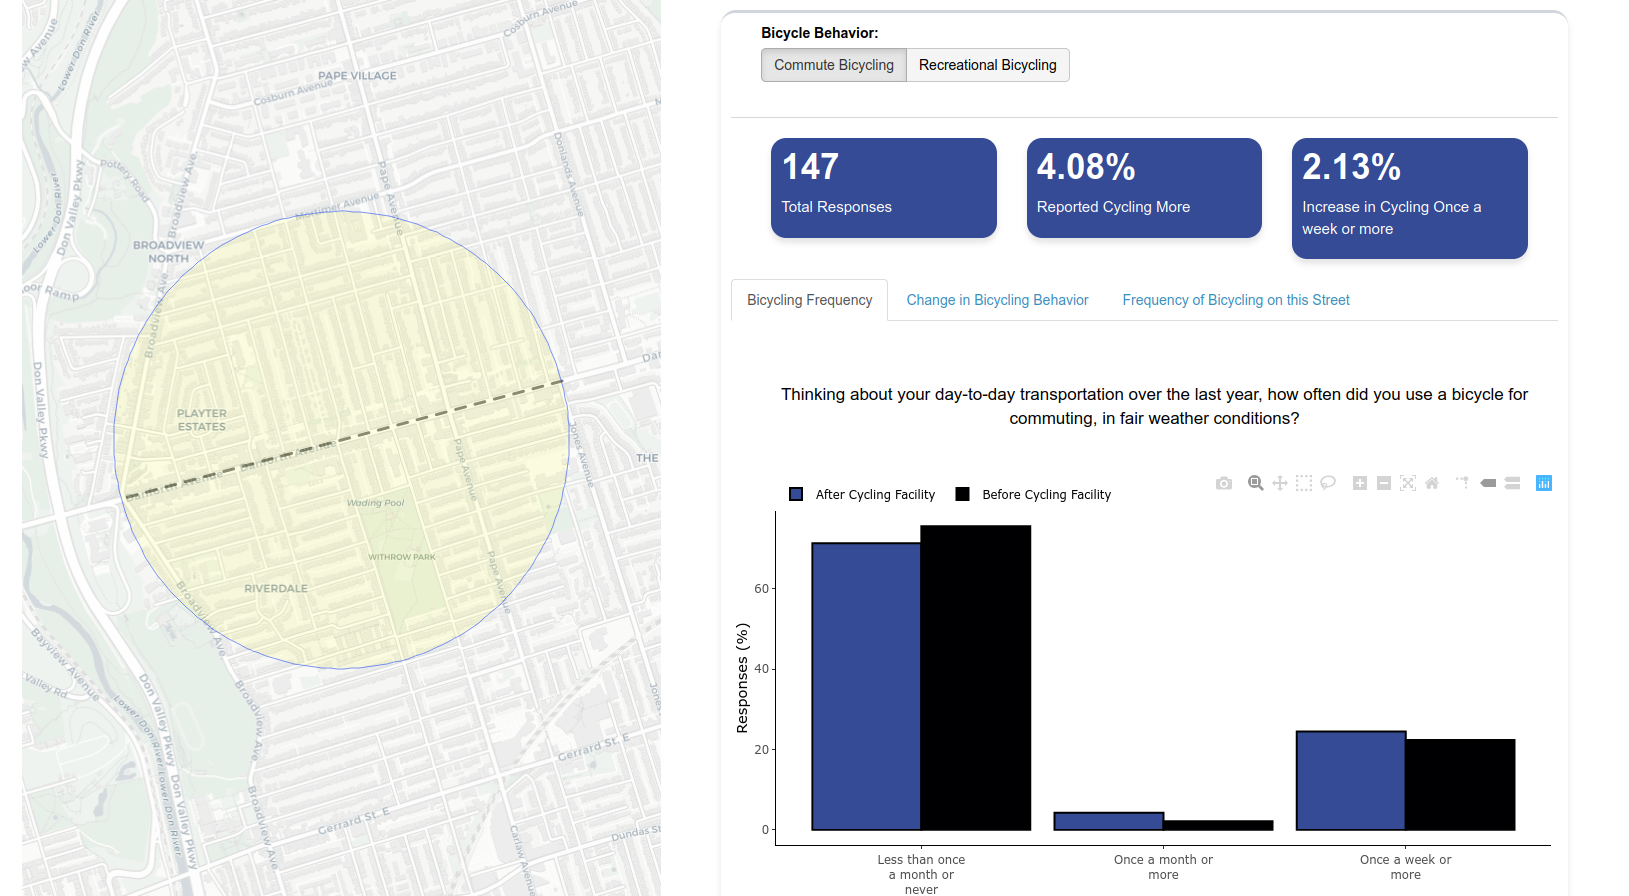
\includegraphics[width=0.95\linewidth]{images/ryerson_cycle_danforth.png}
	\end{figure}
	
	\tiny\url{https://transformlab.shinyapps.io/CyclingInGTHA/}
	
\end{frame}



\begin{frame}
	
	\textbf{Reducing barriers to cycling:} Building safe and comfortable infrastructure 
	
	\begin{figure}
		\centering
		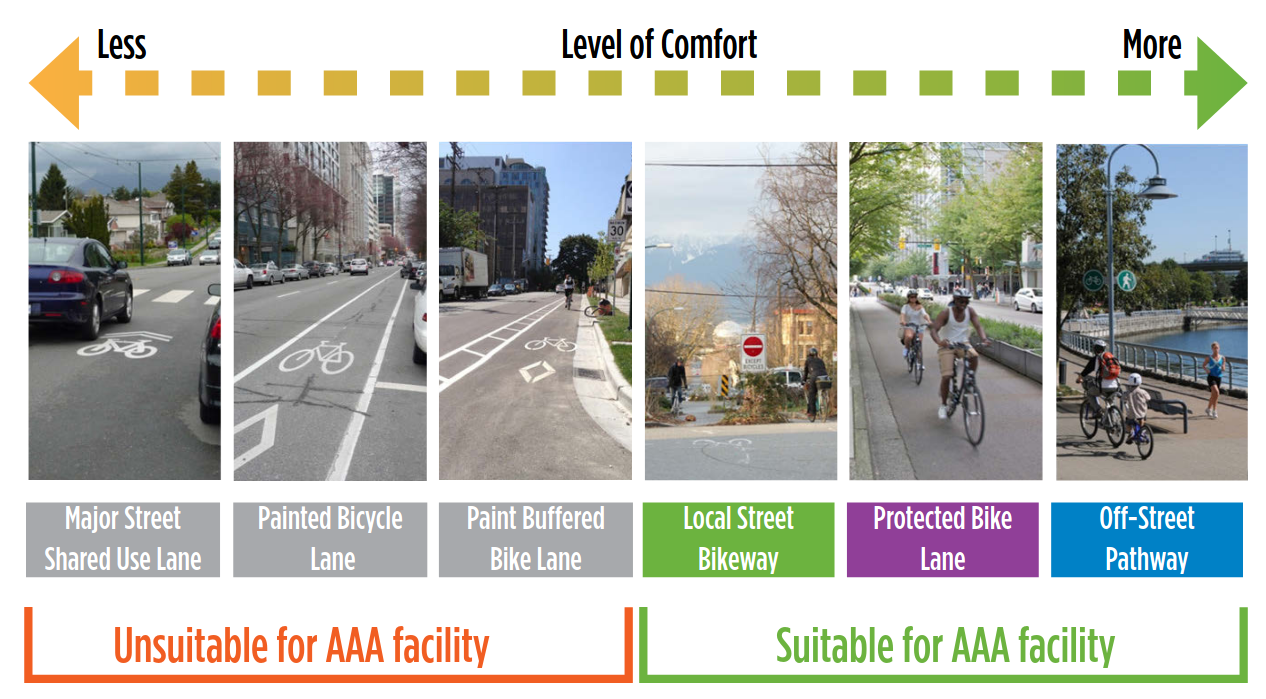
\includegraphics[width=0.85\linewidth]{images/bike_inf_comfort.png}
	\end{figure}

	\small{"The City of Vancouver has a vision to make cycling safe,
		convenient, comfortable and fun for all ages and abilities
		(AAA)"}
	\vspace{2mm}
	
	\tiny\url{https://vancouver.ca/files/cov/design-guidelines-for-all-ages-and-abilities-cycling-routes.pdf}
	
\end{frame}










\begin{frame}
	
	\textbf{Reducing barriers to cycling:} Available and safe bicycle parkring
	
	\begin{figure}
		\centering
		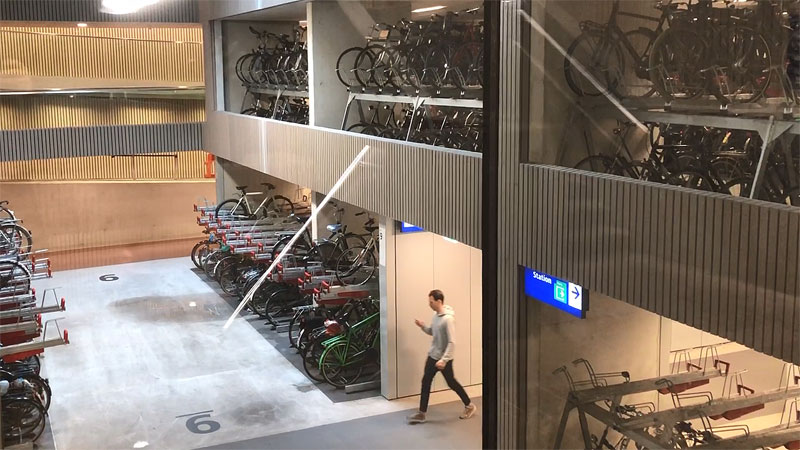
\includegraphics[width=0.85\linewidth]{images/bike_parking_neth.jpg}
	\end{figure}
	
	\tiny\url{https://bicycledutch.wordpress.com/2019/08/20/finally-fully-open-utrechts-huge-bicycle-parking-garage/}
	
\end{frame}



\begin{frame}
	
	\textbf{Reducing barriers to cycling:} Bike escalators in Norway
	
	\begin{figure}
		\centering
		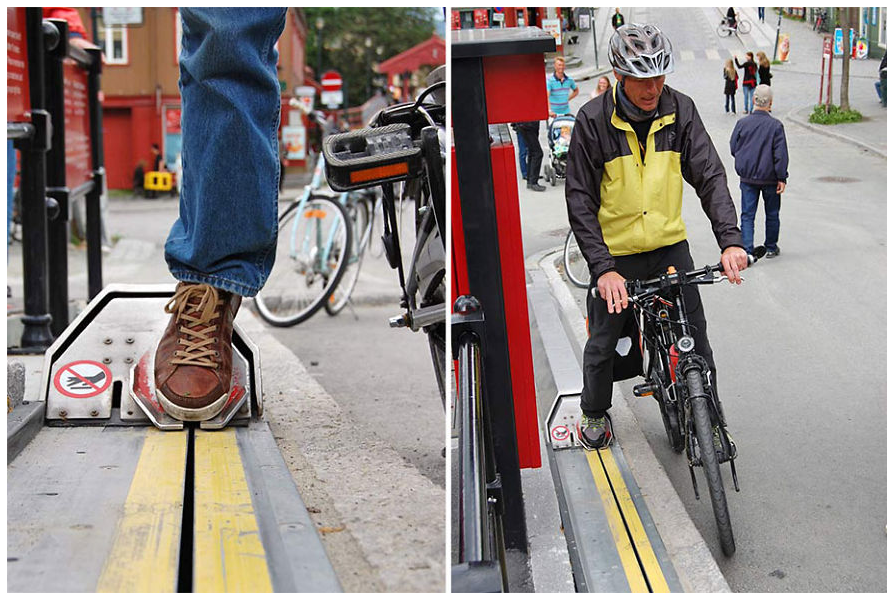
\includegraphics[width=0.85\linewidth]{images/norway_bike_escalator.png}
	\end{figure}
	
	\tiny\url{https://www.boredpanda.com/bicycle-escalator-cyclocable-trondheim-norway/?utm_source=duckduckgo&utm_medium=referral&utm_campaign=organic}
	
\end{frame}





\begin{frame}
	
	\textbf{Reducing barriers to cycling:} Traffic calming
	
	\begin{figure}
		\centering
		\includegraphics[width=0.75\linewidth]{images/wellington.jpg}
	\end{figure}
	
\end{frame}




\begin{frame}
	
	\textbf{Vision Zero:} 
	

	
\end{frame}

% lower speed limits, traffic enforcement, red light cameras

% traffic signals and pedestrian crossings

\begin{frame}
	
	Safer Streets - Leading Pedestrian Interval (i.e. Pedestrian Head Start Signal)
	
\end{frame}

% raised ped crossing

% narrower car lanes - snow example

% chicanes, curb extensions, crossing islands

% city example - e.g. site intersection "diet"

% pavement vs asphalt

% woonerf




\begin{frame}
	
	\textbf{Complete Streets:} 
	
	
	
\end{frame}






\begin{frame}
	
	\textbf{Street Design Activity}
	
\end{frame}



\begin{frame}
	
	Network Connectivity
	
\end{frame}



\begin{frame}
	
	Super blocks (limit car access)
	
	e.g. blocking auto access, but not bikes
	
\end{frame}



\begin{frame}
	
	15-minute cities
	
	Land-use
	
	"Complete" communities
		
\end{frame}




\begin{frame}
	\textbf{Next Week} 
	
	\vspace{4mm}
	
	Public Transit
	
	\begin{itemize}
				
		
		\item etc.
				
		
	\end{itemize}
	
\end{frame}




\end{document}